\chapter{Goals and Use Cases}
\label{ch:Goals and Use Cases}


\section{Goals}
\paragraph{}
In this section, we describe the goals of the project.


\paragraph{}
The structure of the project consists of a component that manages and orchestrates the network (MANO) and NSD that specify the network service to be created and it is a collection of configuration documents which determines how the network service is comprised in terms of VNFs.


\paragraph{}
The main goal of the project is to build three work packages:

\begin{enumerate}
	\item \textbf{Service Descriptor Translator (SDT):} SDT translates NSDs between schema of different MANO frameworks. The translator is required when there is a need to deploy the services across different MANO frameworks.
	
	\item \textbf{Service Descriptor Splitter (SDS):} In order to deploy a network service over different MANO instances, splitter is required to split the NSD into relevant MANO framework specific NSDs.
	
	
	\item \textbf{MANO Scalability Support:} Adaptor is necessary if more than one instance of MANO framework is needed, i.e,  adaptor allows interaction between different instances of MANO frameworks. It also exposes the underlying MANO service instantiation interfaces and retrieves monitoring information about the service status.
\end{enumerate}

\begin{figure}
	\centering
	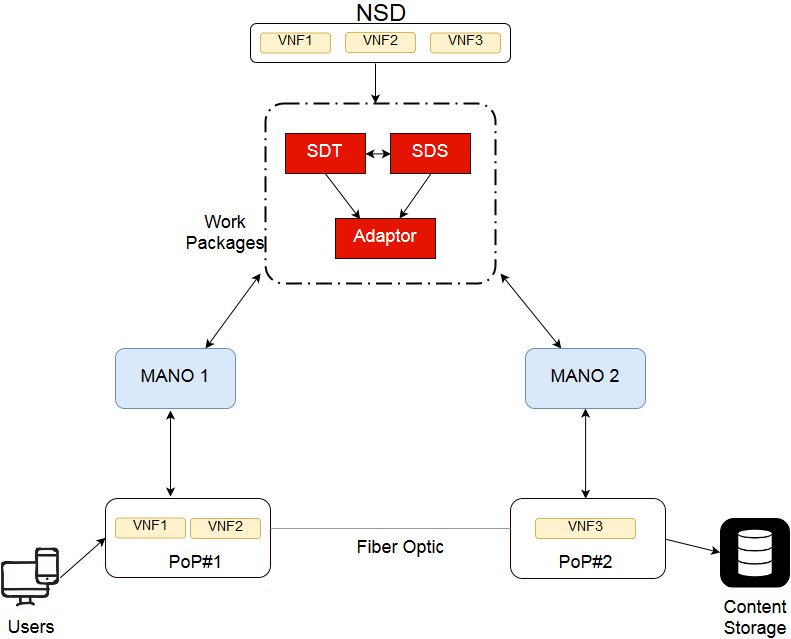
\includegraphics[width=0.7\linewidth]{figures/Structure_Updated1}
	\caption{This figure visualizes the structure of the project. }
	\label{fig:structureupdated1}
\end{figure}
\todo[inline]{Should the figure \ref{fig:structureupdated1} be generalised as client-server?}


\newpage
\section{Use Cases}

\subsection{Cross MANO Framework interaction}
\paragraph{}

As a matter of fact, the MANO frameworks used by every network service provider varies from one another. NSD translation enables the deployment of network services that is in accordance with the intended framework.

For instance : If an operator uses Sonata framework and another operator uses OSM framework, the NSD schemas for both the frameworks will be different. Using the solutions of translation and splitting, network services can be deployed and orchestrated across different MANO implementations.

\subsection{Hierarchical orchestration}
\paragraph{}
By implementing MANO adaptor , dynamic instantiation and inter-operability between different MANO frameworks can be achieved. As a result of this goal, operators will be able to scale up and scale down the resources as and when required. Also, the operator will be able to handle the resources in an efficient manner. 
When there is a high demand for network service, the operator can explore options to include additional MANO instances to mitigate the traffic load on a single MANO instance. The resources can be provisioned based on the number of requests. This helps the operator in extending their profitability. 

\todo[inline]{Please suggest other use-cases that could be included.}























